\documentclass[officiallayout]{tktla}
%\documentclass[officiallayout,a4frame]{tktla}
\usepackage[utf8]{inputenc}
\usepackage{latexsym}
\usepackage{graphicx}
\usepackage[
  backend=biber,
  bibstyle=ieee,
  citestyle=numeric-comp,
    sortlocale=en_US,
    natbib=true,
    url=false, 
    doi=true,
    eprint=false
]{biblatex}
\usepackage{software-biblatex}
\usepackage{pdfpages}
\usepackage[hidelinks]{hyperref}

% For thesis papers section
\usepackage{geometry}
\def \dvWHITE{white}
\def \dvBLACK{black}
\def \dvBLUE{blue}
\def \dvGREEN{green}
\def \dvheight{231pt}
% Creates black box with the text given as first parameter in white
\newcommand\note[3] {\marginpar{\vspace{#2}\colorbox{#3}{\parbox[c][\dvheight][t]{34.8pt}{\vspace{0.3cm}\color{white}\centering\Huge{\textbf{#1}}}}}}

% Footnotes without numbering
\let\svthefootnote\thefootnote

\addbibresource{maklin2022.bib}

\title{Probabilistic methods for \\ plate sweep metagenomics}
\author{Tommi Mäklin}
\authorcontact{tommi@maklin.fi\par
  https://maklin.fi/}
\pubtime{June}{2022}
\reportno{0}
\isbnpaperback{000-00-0000-0}
\isbnpdf{000-00-0000-0}
\issn{1238-8645}
\issnonline{2814-4031}
\printhouse{Unigrafia}
\pubpages{7} % --- remember to update this! 
% For monographs, the number of the last page of the list of references
% For article-based theses, the number of the last page of the list of
% references of the preamble part + the total number of the pages of
% the original articles and interleaf pages.
\supervisorlist{Antti Honkela, University of Helsinki, Finland \\ \hspace{8pt} Jukka Corander, University of Oslo, Norway}
\preexaminera{Exam Iner, University of Examinations, Exaministan}
\preexaminerb{Read Er, University of Examinations, Exaministan}
\opponent{Oppo Nent, University of Endless Argumentation, The Argumentlands}
\custos{Sea Land, University of Sealand, Sealand}
\generalterms{Algorithms, Experimentation}
\additionalkeywords{genomic epidemiology, plate sweeps, probabilistic modeling, pathogen surveillance, taxonomic profiling, taxonomic binning, metagenomics}
% Computing Reviews 1998 style
%\crcshort{A.0, C.0.0}
%\crclong{
%\item[A.0] Example Category
%\item[C.0.0] Another Example
%}
% Computing Reviews 2012 style
\crclong{
\item Mathematics of computing $\rightarrow$ Probability and statistics $\rightarrow$ Statistical computing
\item Computing applications $\rightarrow$ Biosciences
}

\permissionnotice{
  Doctoral dissertation, to be presented for public examination with 
  the permission of the Faculty of Science of the University of
  Helsinki in \ldots{} on \ldots{} at XX o'clock. Fill in the examination
  venue, date and time into the previous sentence.
}

\newtheorem{theorem}{Theorem}[chapter]
\newenvironment{proof}{\noindent\textbf{Proof.} }{$\Box$}

\begin{document}

\frontmatter

\maketitle

\begin{abstract}
  rewrite \citet{maklin_high-resolution_2021} a \citep{maklin_bacterial_2021}

\end{abstract}

\begin{acknowledgements}
  Olvi (III) \\ \& Koff IVA
   \begin{flushright}
  Rv  rip, June 2022\\
  Tommi Mäklin
  \end{flushright}
\end{acknowledgements}

\tableofcontents

\mainmatter

\chapter{Introduction}

In the past decades research focusing on bacterial pathogens has
largely been driven by analysis of the contents of bacterial genomes
obtained by whole-genome sequencing. Although the price of sequencing
itself has decreased tremendously during this timeframe, most analyses
still rely on using sequence data from pure bacterial cultures created
by isolating a bacterium from an initial mixed culture. Since these
cultures are created by cultivating environmental samples, they
typically contain several distinct bacteria \textemdash and other
microorganisms \textemdash that a thorough analysis would aim to
isolate in a pure culture. In practice, the number of isolations that
can be performed is limited and preparing large numbers of samples for
DNA sequencing rapidly becomes a significant economical barrier even
in well-resourced public health laboratories.

The typical use for sequencing data in public health settings is
genomic epidemiology, where researchers are interested analysing the
genomes of the pathogens to trace their transmission and spread. For
example, comparing mutations in the genomes of a pathogen isolated
from several patients during an epidemic may aid in inferring the
transmission chain by elucidating the short-term evolutionary
history. Similarly the long-term history can be inferred by looking
for larger structural changes, horizontal gene transfer, and
accumulated mutations in genomes assembled from the sequence data. If
the sequencing is performed routinely and the data is made publicly
available, the reporting from several laboratories may be combined to
create an extremely valuable resource for both researchers and
policymakers. However, the vast majority of genomic epidemiological
analyses require high coverage and high quality sequence data to
achieve meaningful resolution, which has translated to dominance of
the expensive pure-colony isolation approach in data generation.

Recently, shotgun metagenomics, where DNA is extracted and sequenced
directly from the original environmental sample, has emerged as a
potential cost-effective alternative to pure whole-genome
sequencing. Although this approach conveniently gets around both the
economic barrier and potential biases introduced by the cultivation
steps, direct sequencing often requires significantly higher
sequencing depths. Sequencing at depths typical to isolate analyses
often results in excess amounts of host DNA and fails to provide
sufficient resolution for the more elusive members of the microbiome
that are present only at low abundances. Due to these factors, shotgun
metagenomics may be difficult to apply in situations where researchers
are only interested in some subset of bacteria but wish to perform
analyses that require high sequencing depth.

When choosing between shotgun metagenomics and isolate sequencing, a
middle-ground can be found in creating the initial mixed culture but
skipping the isolation steps and instead sweeping and sequencing the
mixed culture. Since culture media are available for most clinically
relevant bacteria, this approach allows enrichment of the species of
interest while simultaneously filtering out host DNA, effectively
avoiding the pitfalls in both isolate and shotgun metagenomics by
limiting the diversity of the sample. Accordingly, this approach is
sometimes called limited-diversity metagenomics
\citep{cocker_drivers_2022} but will be referred to as plate sweep
metagenomics in this thesis.

Although both plate sweep metagenomics and shotgun metagenomics
have technically been possible for many years, the development of
computational methods has largely focused on analysing data from pure
cultures. Although some advances have been made in developing
computational tools capable of identifying the taxonomic composition
of a set of reads (taxonomic profiling) or assigning the individual
sequencing reads to their taxonomic origins (taxonomic binning), the
accuracy of these tools is significantly hindered in the presence of
within-species variation. In practice such variation is ubiquitous in
both clinical and envinronmental samples, rendering many of the tools
difficult to use when within-species level information is required.

In this thesis I present research that enables both taxonomic
profiling and binning from either metagenomic or plate sweep
sequencing data using computational methods. While the methods were
initially developed for plate sweeps metagenomics work, I also
demonstrate that they can reliably be applied to whole metagenome
sequencing data as well. Using either of the two approaches to
generate metagenomic sequencing data enables performing completely new
types of analyses which are also briefly covered.

The first two articles included in this thesis contain descriptions of
the aforementioned two methods. The first of these methods, called
mSWEEP, provides a probabilistic model for taxonomic profiling of
bacteria at within-species lineage level based on pseudoalignments
against a set of reference sequences. The second method, mGEMS,
leverages the information from mSWEEP to construct an assignment rule
for taxonomic binning of sequencing reads to bins that correspond to
the lineages. Both methods rely on the fundamentally important insight
that each sequencing read can - and should - pseudoalign and be
assigned to several lineages within the species at once. By combining
the two methods, sequencing data from samples containing several
lineages of the same species can be computationally demixed and used
to obtain results that are nearly indistinguishable from the results
of using isolate data.

While the methods from the first two articles are designed with direct
analysis of sequencing data from mixed cultures in mind, the third
article shows that both methods are applicable even when the initial
plating step is skipped and the sequencing data is derived directly
from an environmental sample. Thus, in the third article I have
analysed such samples from babies born in the UK collected during
their neonatal period and discovered several results showing strong
competition between bacterial species and strains during the initial
colonization of the gut microbiome. More importantly, from a methods
perspective, this analysis shows that mSWEEP and mGEMS provide
(so-far) completely unprecedented levels of resolution in analysis of
metagenomic sequencing data.

Together the three articles in this thesis represent foundational
methodological steps in both opening up high-resolution exploration of
bacterial diversity as well as making such analyses more accessible to
resource-constrained laboratories.

\section{Three approaches to sequencing bacterial DNA}

\begin{figure}[!ht]
  \label{fig:microbiome-sampling-methods}
    \centering
    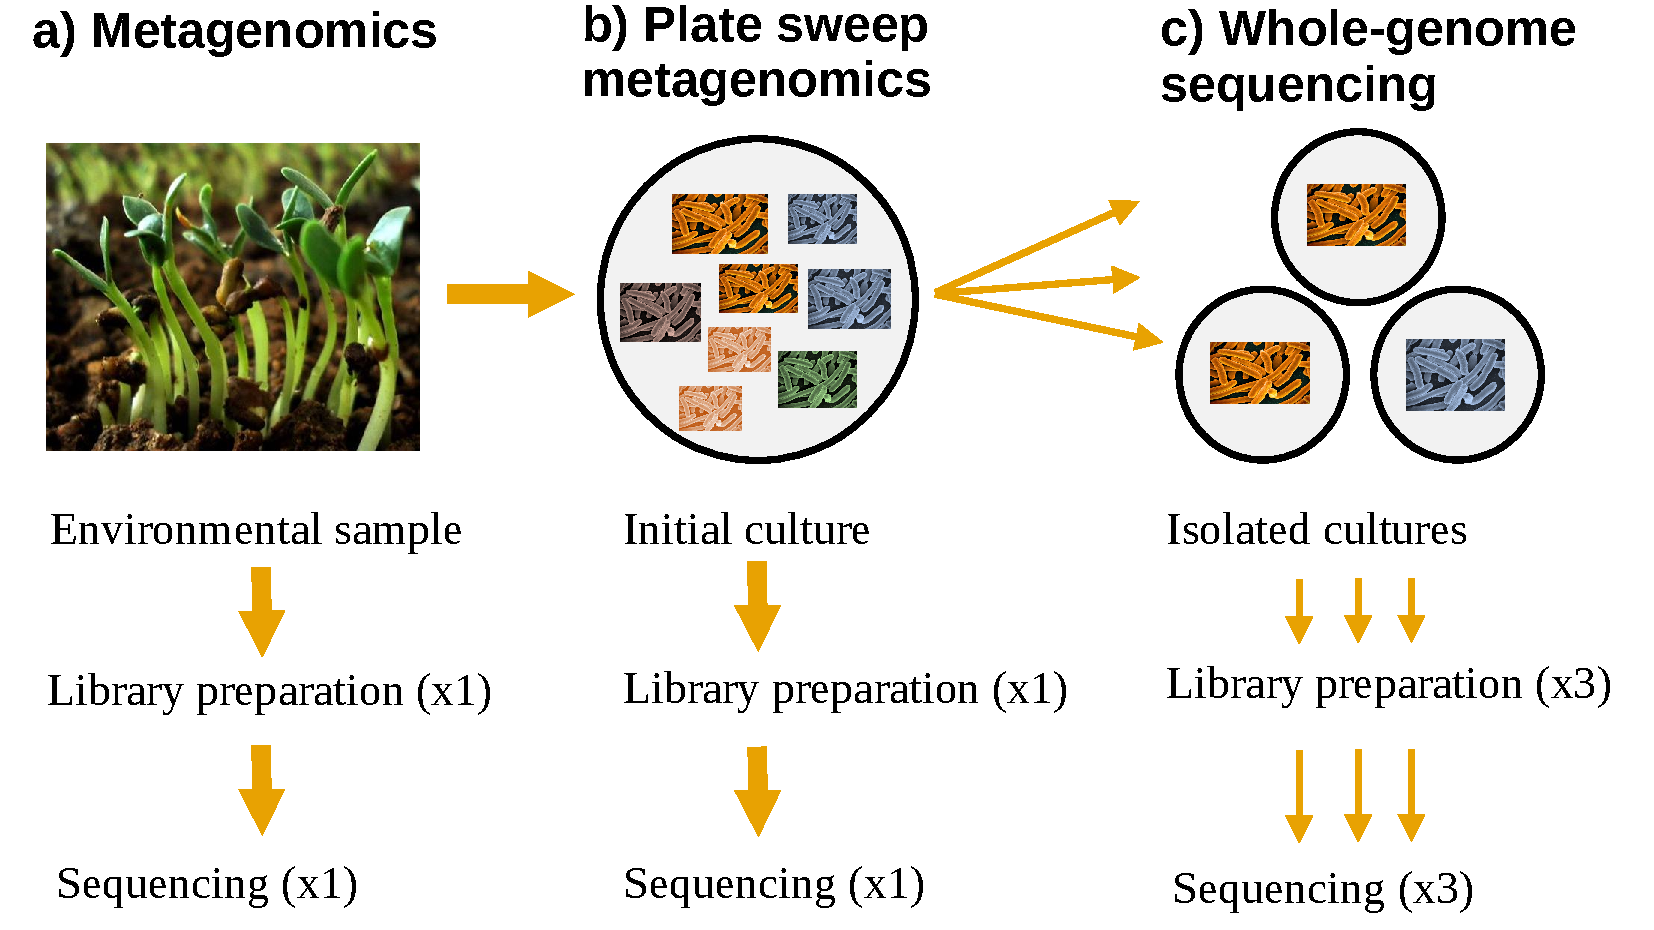
\includegraphics[width=\textwidth,keepaspectratio]{img/sampling/microbiome_sampling_methods.pdf}
    \caption{Different approaches to sequencing bacterial DNA. Panel \textbf{a)} depicts the metagenomic approach, where sequence data is collected directly from the environmental sample. Panel \textbf{b)} depicts the plate sweep metagenomic approach, where the environmental sample is plated on a selective medium and DNA is sequenced from the whole plate. Panel \textbf{c)} depicts the whole-genome sequencing approach, where a subset of visible colonies on the selective medium are picked, cultured again on their own plates, and then sequenced. The orange arrows depict steps that require laboratory work.}
\end{figure} \let\thefootnote\relax\footnote{Figure source: Adapted from \cite{praveera_fenugreek-sprouts} and \cite{niaid_escherichia-coli}. Released under the \href{https://creativecommons.org/licenses/by-sa/4.0}{CC BY-SA 4.0 license}.}
\addtocounter{footnote}{-1}\let\thefootnote\svthefootnote

- Cover the three approaches to data collection presented in \ref{fig:microbiome-sampling-methods}.

- What are the strengths and weaknessess of each approach? Why do we want to favour approaches b) and a)?

- Some coverage of previous literature regarding the approaches.

\section{Analysing metagenomic sequence data}

- Cover previous work in metagenome data analysis: metagenome
assemblers, metagenome binners, metaphlan, strainphlan, strainGE,
etc. Also briefly touch 16S sequencing.

- Introduce our approach and cover why it is different from the previous approaches (Gerry's paper is especially useful here).

- Cover some applications and results from literature.

\section{Contributions}

This thesis comprises three publications covering both mSWEEP and
mGEMS as well as a third article demonstrating their application to
whole-genome shotgun metagenomic sequencing data. The first two
publications are accompanied by software implementations. The third
article is more applied in nature, exploring in more detail the types
of analyses enabled by the first two papers.

\subsection*{Paper I \textemdash High-resolution sweep metagenomics using fast probabilistic inference}
By \underline{Tommi Mäklin}, Teemu Kallonen, Sophia David, Christine J
Boinett, Ben Pascoe, Guillaume Méric, David M Aanensen, Edward J Feil,
Stephen Baker, Julian Parkhill, Samuel K Sheppard, Jukka Corander, and
Antti Honkela. Published in \textit{Wellcome Open Research} (2021),
5:14, doi: 10.12688/wellcomeopenres.15639.2.

In the first paper, we presented and benchmarked the mSWEEP method for
taxonomic profiling of sequencing data containing multiple strains
from the same bacterial species. My contributions included development
and implementation of the method, designing the benchmarks and
comparisons with similar methods, running all analyses with mSWEEP,
writing the manuscript, and to reviewing and editing the article.

Software implementation of the ideas presented in Paper I is
available from GitHub at
\href{https://github.com/PROBIC/mSWEEP}{PROBIC/mSWEEP} (latest
version). The latest version at the time of writing is archived and
available in Zenodo \citep{maklin_mSWEEP}.

\subsection*{Paper II \textemdash Bacterial genomic epidemiology with mixed samples}
By \underline{Tommi Mäklin}, Teemu Kallonen, Jarno Alanko, Ørjan
Samuelsen, Kristin Hegstad, Veli Mäkinen, Jukka Corander, Eva Heinz,
and Antti Honkela. Published in \textit{Microbial Genomics} (2021)
7.11, doi: 10.1099/mgen.0.000691.

The second paper continued to build upon mSWEEP by developing an
algorithm for taxonomic binning at within-species variation level,
called mGEMS. I contributed to the development of both the mGEMS
binning algorithm and the full mGEMS pipeline, designing the synthetic
and the \textit{in vitro} benchmark experiments, running the analyses
and creating the visualisations, interpreting the results and writing
the article, and to reviewing and editing the article.

Software implementation of the ideas presented in Paper II is
available from GitHub at
\href{https://github.com/PROBIC/mGEMS}{PROBIC/mGEMS} (latest version).
The latest version at the time of writing is archived and available in
Zenodo \citep{maklin_mSWEEP}.

\subsection*{Paper III \textemdash Strong pathogen competition in neonatal gut colonization}
By \underline{Tommi Mäklin}, Harry Thorpe, Anna Pöntinen, Rebecca
Gladstone, Alan McNally, Ørjan Samuelsen, Pål Johnsen, Trevor Lawley,
Antti Honkela, and Jukka Corander. Awaiting peer-review; available
from \textit{bioRxiv} (2022), doi: XXX.XX/XXX.XXX.XXX.

Description...

The author...

\section{Structure}

This is a sample sentence that should look like normal text, and this
is another. This is a sample sentence that should look like normal
text, and this is another. This is a sample sentence that should look
like normal text, and this is another. This is a sample sentence that
should look like normal text, and this is another. This is a sample
sentence that should look like normal text, and this is another. 

\chapter{Mixture modeling of sequence data}

Something about bacterial pathogens are hard to classify taxonomically
and have weird genomes with weird plasmids and stuff.  Lineages are
much much nicer to work with

- Add results from Gibbs sampler vs variational inference experiments.

This is a sample sentence that should look like normal text, and this
is another. This is a sample sentence that should look like normal
text, and this is another:
\[ S = \sum_{i=0}^{\infty} a^2 \]
This is a sample sentence that should look like normal text, and this
is another.\footnote{A sample footnote.}

\begin{theorem}
This is a sample sentence ($x=x+2$) that should look like normal text,
and this is another. This is a sample sentence that should look like
normal text, and this is another. This $x$ is a sample sentence $y$
that should look like normal text 32, and this is another.
\end{theorem}

\begin{proof}
This is a sample sentence that should look like normal text, and this
is another. This is a sample sentence that should look like normal
text, and this is another.
\end{proof}

\begin{theorem}
This is a sample sentence that should look like normal text,
and this is another:
\[ y = x+3 \]
\end{theorem}

\begin{proof}
This is a sample sentence.
\end{proof}

\chapter{High-resolution metagenomics}

cite \citet{tonkin-hill_pneumococcal_2022} for rigorous proof that
mSWEEP/mGEMS can recover cocolonization by several strains that is
overlooked by isolate sequeuncing.

Define plate sweeps

Pretty picture of how to use them

Something about metagenomics is nice in that we dont just sequence one
nice things but many nice things

Introducing mSWEEP/mGEMS \& how these tools enable new directions in research.

Figure~\ref{fig:examplefigure} shows an example on how figures in the 
eps format can be included into the text. It gives an example on how 
figures in the eps format can be included into the text. It gives 
an example on how figures in the eps format can be included into the text.

\chapter{Metagenomic epidemiology}

Something about wgs and genomic epidemiology can do lots of cool stuff
to identify contaminated cucumbers or track covid

\printbibliography[heading=bibintoc]

\chapter*{Included papers\markboth{Included papers}{}}
\addcontentsline{toc}{chapter}{Included papers}

\subsection*{Paper I \textemdash High-resolution sweep metagenomics using fast probabilistic inference}
By \underline{Tommi Mäklin}, Teemu Kallonen, Sophia David, Christine J
Boinett, Ben Pascoe, Guillaume Méric, David M Aanensen, Edward J Feil,
Stephen Baker, Julian Parkhill, Samuel K Sheppard, Jukka Corander, and
Antti Honkela. Published in \textit{Wellcome Open Research} (2021), 5:14
(https://doi.org/10.12688/wellcomeopenres.15639.2).

\subsection*{Paper II \textemdash Bacterial genomic epidemiology with mixed samples}
By \underline{Tommi Mäklin}, Teemu Kallonen, Jarno Alanko, Ørjan
Samuelsen, Kristin Hegstad, Veli Mäkinen, Jukka Corander, Eva Heinz,
and Antti Honkela. Published in \textit{Microbial Genomics} (2021)
7.11 (https://doi.org/10.1099/mgen.0.000691).

\subsection*{Paper III \textemdash Strong pathogen competition in neonatal gut colonization}
By \underline{Tommi Mäklin}, Harry Thorpe, Anna Pöntinen, Rebecca
Gladstone, Alan McNally, Ørjan Samuelsen, Pål Johnsen, Trevor Lawley,
Antti Honkela, and Jukka Corander. Awaiting peer-review; available
from \textit{bioRxiv} (2022) (https://doi.org/10.1099/mgen.0.000691).

%% \documentclass[officiallayout]{tktla}
%% \usepackage[utf8]{inputenc}
%% \usepackage{pdfpages}
%% % This package sets the margin width 
%% % (change "right" if you want them wider, but then change the 34.8pt in \note bigger too)
%% \usepackage[top=1.2in, bottom=1.5in, left=1in, right=1.6cm]{geometry}
%% \def \dvWHITE{white}
%% \def \dvBLACK{black}
%% \def \dvBLUE{blue}
%% \def \dvGREEN{green}
%% %%.72 = marker width§
%% %% 138,6: height 
%% % Use this if you have 5 articles
%% %\def \dvheight{138.6pt}
%% % Use this if you have 6 articles
%% \def \dvheight{115.5pt}
%% % Creates black box with the text given as first parameter in white
%% \newcommand\note[3] {\marginpar{\vspace{#2}\colorbox{#3}{\parbox[c][\dvheight][t]{34.8pt}{\vspace{0.3cm}\color{white}\centering\Huge{\textbf{#1}}}}}}

%% % This overlays a white box to make black box narrower, but it's not needed anymore with geometry package changing margin width
%% %\newcommand\notee[2]{\marginpar{\vspace{#1}\colorbox{#2}{               \parbox[c][\dvheight][t]{11.8pt}{              \color{white}\centering\Huge{\textbf{$\ $}}}}}}

%% \pagestyle{empty}
%% \begin{document}


\newgeometry{top=1.2in, bottom=1.5in, left=1in, right=1.6cm}

% ******************************************************************************
\chapter*{Paper I}\thispagestyle{plain}
\addcontentsline{toc}{section}{High-resolution sweep metagenomics using fast probabilistic inference}

\note{I}{-222pt}{black}
%\notee{-222pt}{\dvWHITE}

% Here it's not necessary to draw the following boxes to position right,
% and drawing them occasionally creates unwanted gray lines

%\note{II}{-100pt}{\dvWHITE}
%\notee{-126.5pt}{\dvWHITE}

%\note{III}{-5pt}{\dvWHITE}
%\notee{-126.5pt}{\dvWHITE}

%\note{IV}{-5pt}{\dvWHITE}
%\notee{-126.5pt}{\dvWHITE}

%\note{V}{-5pt}{\dvWHITE}
%\notee{-126.5pt}{\dvWHITE}

%\note{VI}{-5pt}{\dvWHITE}
%\notee{-126.5pt}{\dvWHITE}

\vspace{80pt}
% The names of the authors
\underline{Tommi Mäklin}, Teemu Kallonen, Sophia David, Christine J
Boinett, Ben Pascoe, Guillaume Méric, David M Aanensen, Edward J Feil,
Stephen Baker, Julian Parkhill, Samuel K Sheppard, Jukka Corander, and
Antti Honkela.

\vspace{10pt}
% Title of the 1st paper
\noindent\textbf{High-resolution sweep metagenomics using fast probabilistic inference}

\vspace{10pt}
% Bibliographical information of the paper, for example, of a conference paper
\noindent In
\emph{Wellcome Open Research},
\\vol. 5 issue 14, 2021.

\vspace{60pt}
% Copyright information, if the publisher is, for example, ACM
\noindent Copyright \textcopyright\ 2021 Mäklin T et al. This is an
open access article distributed under the terms of the Creative
Commons Attribution License, which permits unrestricted use,
distribution, and reproduction in any medium, provided the original
work is properly cited.

\cleardoublepage
% Including the original publication
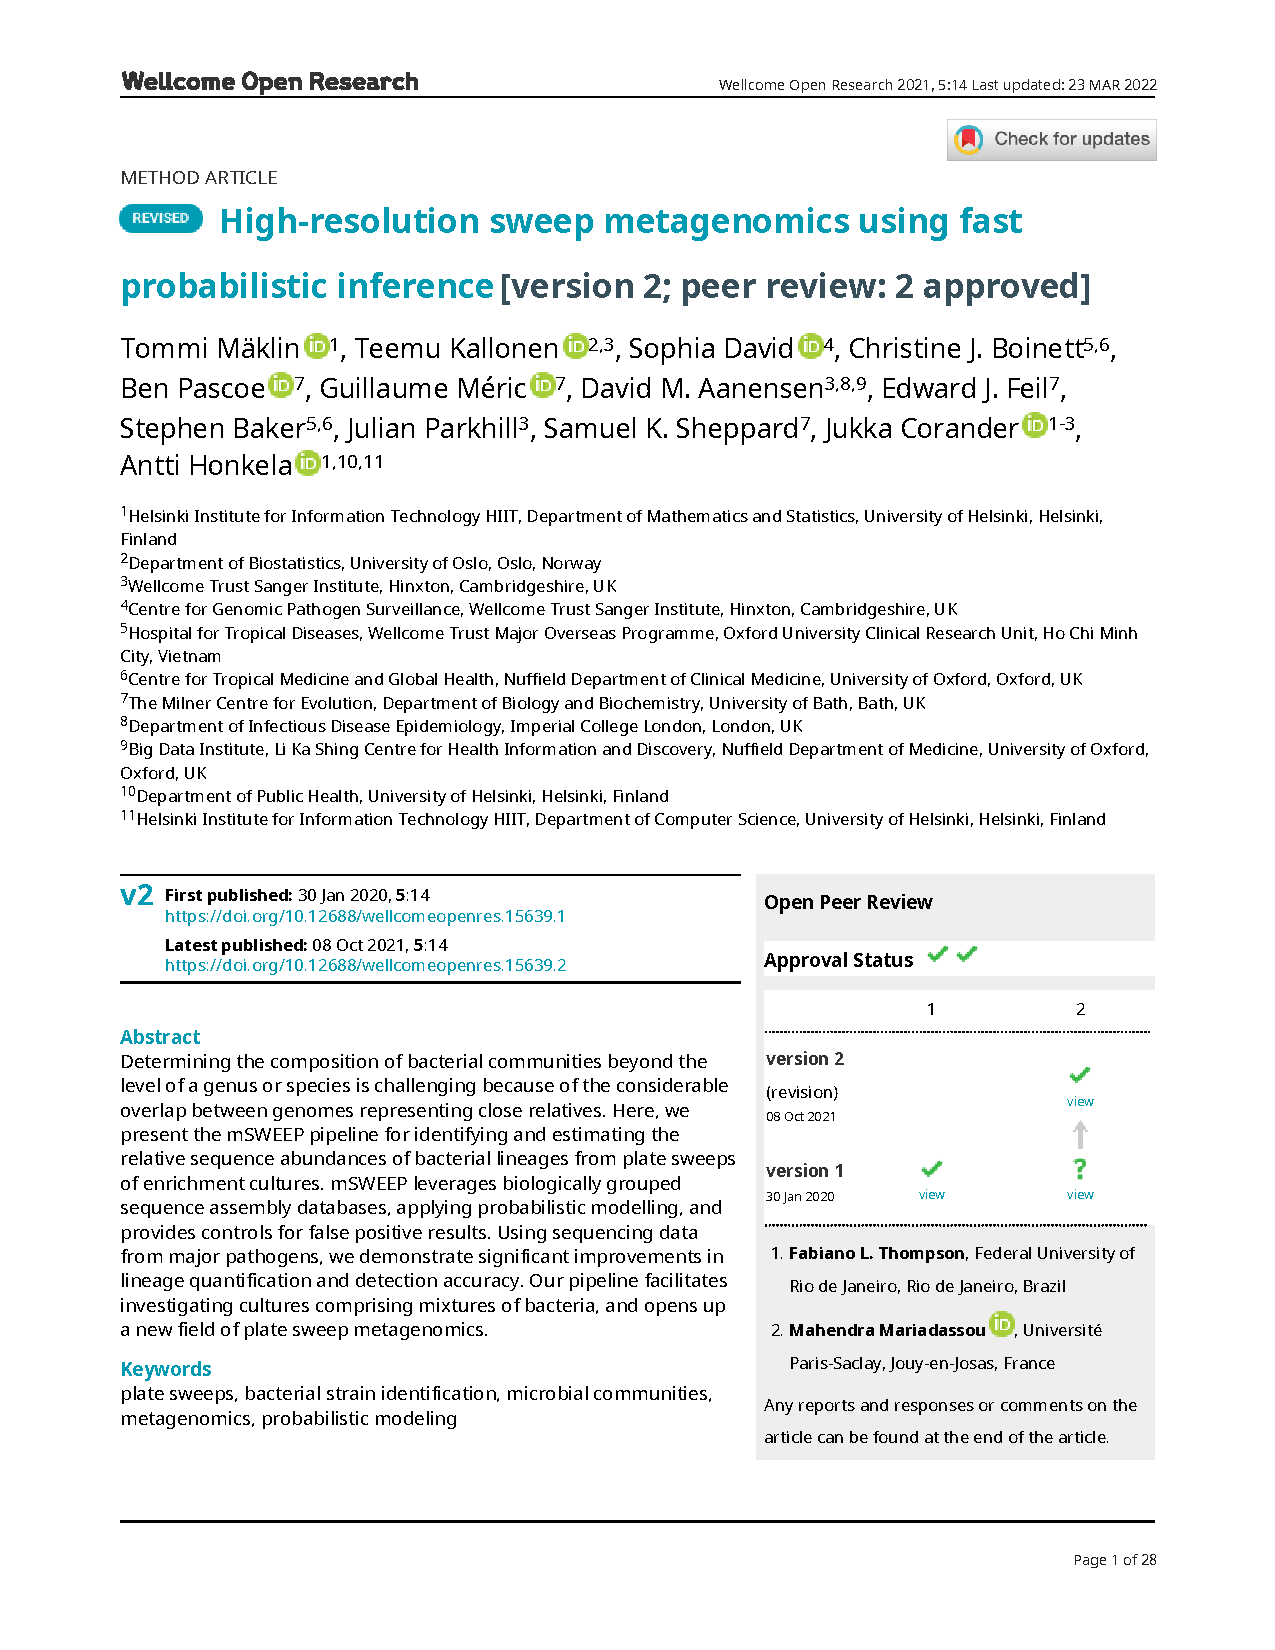
\includepdf[pages=-]{papers/maklin_high-resolution_2021.pdf}


% ******************************************************************************


\chapter*{Paper II}\thispagestyle{plain}
\addcontentsline{toc}{section}{Bacterial genomic epidemiology with mixed samples}

\note{I}{-222pt}{\dvWHITE}
%\notee{-222pt}{\dvWHITE}

\note{II}{-5pt}{black}
%\notee{-126.5pt}{\dvWHITE}

\note{III}{0pt}{\dvWHITE}
%\notee{-126.5pt}{\dvWHITE}

%% \note{IV}{-5pt}{\dvWHITE}
%% %\notee{-126.5pt}{\dvWHITE}

%% \note{V}{-5pt}{\dvWHITE}
%% %\notee{-126.5pt}{\dvWHITE}

%% \note{VI}{-5pt}{\dvWHITE}
%% %\notee{-126.5pt}{\dvWHITE}

\vspace{80pt}

% Here are the names of the authors
\underline{Tommi Mäklin}, Teemu Kallonen, Jarno Alanko, Ørjan
Samuelsen, Kristin Hegstad, Veli Mäkinen, Jukka Corander, Eva Heinz,
and Antti Honkela.

\vspace{10pt}
% Title of the 2nd paper
\noindent\textbf{Bacterial genomic epidemiology with mixed samples}

\vspace{10pt}
% Bibliographical information of the paper, for example, of a conference paper
\noindent In 
\emph{Microbial Genomics}, 
\\vol. 7 issue 11, 2021.

\vspace{60pt}
% Copyright information, for example, if the publisher is Springer
\noindent Copyright \textcopyright\ The Authors. This is an
open-access article distributed under the terms of the Creative
Commons Attribution License. This article was made open access via a
Publish and Read agreement between the Microbiology Society and the
corresponding author’s institution.

\cleardoublepage
% Including the original publication
\includepdf[pages=-]{papers/maklin_bacterial_2021.pdf}

% ******************************************************************************


\chapter*{Paper III}\thispagestyle{plain}
\addcontentsline{toc}{section}{Strong pathogen competition in neonatal gut colonization}

\note{I}{-222pt}{\dvWHITE}
%\notee{-222pt}{\dvWHITE}

\note{II}{-5pt}{\dvWHITE}
%\notee{-126.5pt}{\dvWHITE}

\note{III}{0pt}{black}
%\notee{-126.5pt}{\dvWHITE}

%% \note{IV}{-5pt}{\dvWHITE}
%% %\notee{-126.5pt}{\dvWHITE}

%% \note{V}{-5pt}{\dvWHITE}
%% %\notee{-126.5pt}{\dvWHITE}

%% \note{VI}{-5pt}{\dvWHITE}
%% %\notee{-126.5pt}{\dvWHITE}

\vspace{80pt}
% Here are the names of the authors
\underline{Tommi Mäklin}, Harry Thorpe, Anna Pöntinen, Rebecca Gladstone, Alan McNally, Ørjan
Samuelsen, Pål Johnsen, Trevor Lawley, Antti Honkela, and Jukka Corander.

\vspace{10pt}
% Title of the 3rd paper
\noindent\textbf{Strong pathogen competition in neonatal gut colonization}

\vspace{10pt}
% Bibliographical information of the paper, for example, a submitted paper
\noindent Submitted, preprint available from \emph{bioRxiv}.

\vspace{60pt}
%Copyright information, when the authors have the copyright of the paper
\noindent
The copyright holder for this preprint is the author/funder, who has
granted bioRxiv a license to display the preprint in perpetuity. It is
made available under a CC-BY 4.0 International license.

\cleardoublepage
% Including the original publication
%\includepdf[pages=-]{Publication_name_3.pdf}



% ******************************************************************************


%% \chapter*{Paper IV}\thispagestyle{empty}
%% \note{I}{-222pt}{\dvWHITE}
%% %\notee{-222pt}{\dvWHITE}

%% \note{II}{-100pt}{\dvWHITE}
%% %\notee{-126.5pt}{\dvWHITE}

%% \note{III}{-5pt}{\dvWHITE}
%% %\notee{-126.5pt}{\dvWHITE}

%% \note{IV}{-5pt}{black}
%% %\notee{-126.5pt}{\dvWHITE}

%% \note{V}{-5pt}{\dvWHITE}
%% %\notee{-126.5pt}{\dvWHITE}

%% \note{VI}{-5pt}{\dvWHITE}
%% %\notee{-126.5pt}{\dvWHITE}

%% \vspace{80pt}
%% % Here are the names of the authors
%% John Doe, Jane Doe, and John Smith

%% \vspace{10pt}
%% % Title of the 4th paper
%% \noindent\textbf{This is the title of the 4th paper}

%% \vspace{10pt}
%% % Bibliographical information of the paper, for example, of a journal paper
%% \noindent
%% In \emph{Journal name}, \\Volume xx, 20ZZ, pages XX-YY.

%% \vspace{60pt}
%% % Copyright information, when the authors have the copyright
%% \noindent Copyright \textcopyright\ The Authors.

%% \cleardoublepage
%% % Including the original publication
%% \includepdf[pages=-]{Publication_name_4.pdf}

% ******************************************************************************

\restoregeometry

%\end{document}


\end{document}
